\documentclass[../main.tex]{subfiles}
\begin{document}
	
	\section{Lista 6}
	\begin{exercicio}{1}
		(T. Apostol; seção 10.5; exercícios 1, 4 e 9)
		
		Desenhar em ambiente computacional o campo e o caminho. Resolver manualmente e computacionalmente a integral de linha. Escolha 2 (ou mais) pontos da curva para indicar ambos os vetores do integrando: tangente da curva e o campo no ponto específico.
		
		\begin{enumerate}
			\item[1.] $f(x,y)=(x^2-2xy)\textbf{i} + (y^2-2xy)\textbf{j}$, de $(-1,1)$ até $(1,1)$ ao longo da parábola $y=x^2$.
			\item[4.] $f(x,y)=(x^2+y^2)\textbf{i}+(x^2-y^2)\textbf{j}$, de $(0,0)$ até $(2,0)$ ao longo da curva $y=1-|1-x|$.
			\item[9.] $\int_C (x^2-2xy)dx+(y^2-2xy)dy$, onde $C$ é o caminho de $(-2,4)$ até $(1,1)$ ao longo da parábola $y=x^2$.   
		\end{enumerate}
	\end{exercicio}
	\begin{solucao}
		\begin{enumerate}
			\item[1.] Seja $\alpha(t)=(t,t^2)\Rightarrow \alpha'(t)=(1,2t)$, onde $\alpha$ é parametrização da parábola, com $-1<t<1$. Assim, temos que
			\begin{align*}
				\int_C f\, d\alpha
				&=\int_{-1}^1 f(\alpha(t))\cdot \alpha'(t)\, dt\\
				&=\int_{-1}^1 (t^2-2t^3, t^4-2t^3)\cdot (1,2t)\, dt\\
				&=\int_{-1}^1 t^2-2t^3+2t^5-4t^4\, dt \\
				&=\bigg[\frac{t^3}{3}-2\frac{t^4}{4}+2\frac{t^6}{6}-4\frac{t^5}{5}\bigg]_{-1}^1\\
				&=\frac{1-(-1)}{3}-\frac{(1-1)}{2}+\frac{1-1}{3}-4\frac{1-(-1)}{5}\\
				&=\frac{2}{3}-\frac{8}{5}\\
				&=-\frac{14}{15}
			\end{align*}
			Abaixo segue o campo e o caminho ilustrados em ambiente computacional, bem como 3 pontos escolhidos da curva, com seus respectivos vetores tangentes e do campo.
			\begin{center}
				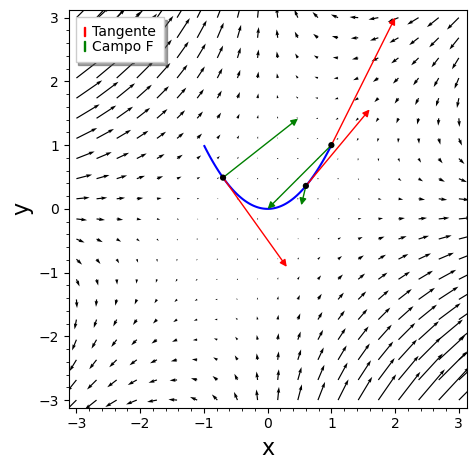
\includegraphics[width=0.25\textwidth]{imagens/lista06/picture_lista06_q01_item01.png}
				\captionof{figure}{Campo vetorial $f$ e caminho $C$}
			\end{center}
			\item[4.] Seja $\alpha(t)=(t,1-|1-t|)$, onde $\alpha$ é parametrização da curva $C$, com $0<t<2$. Devido à função módulo precisamos dividir essa curva $C$ em $C_1$ e $C_2$, de parametrizações $\alpha_1$ e $\alpha_2$ respectivamente, onde
			\[
			\begin{cases} \alpha_1(t)=(t,1-(1-t)), 0<t\leq 1 \\ \alpha_2(t)=(t,1+(1-t)), 1<t<2 \end{cases}\Rightarrow \begin{cases} \alpha_1(t)=(t,t), 0<t\leq 1 \\ \alpha_2(t)=(t,2-t))), 1<t<2 \end{cases}
			\]
			Além disso, note que $\alpha_1'(t)=(1,1)$ e $\alpha_2'(t)=(1,-1)$.
			Assim, temos que
			\begin{align*}
				\int_C f\, d\alpha
				&=\int_{C_1} f\, d\alpha_1+\int_{C_2} f\, d\alpha_2\\
				&=\int_{0}^1 f(\alpha_1(t))\cdot \alpha_1'(t)\, dt+\int_{1}^2 f(\alpha_2(t))\cdot \alpha_2'(t)\, dt\\
				&=\int_{0}^1 (t^2+t^2, t^2-t^2)(1,1)\, dt+\int_{1}^2 (t^2+(2-t)^2, t^2-(2-t)^2)(1,-1)\, dt\\
				&=\int_{0}^1 2t^2\, dt + \int_{1}^2 2(t^2-4t+4)\, dt \\
				&=2\bigg[\frac{t^3}{3}\bigg]_{0}^1+2\bigg[\frac{t^3}{3}-4\frac{t^2}{2}+4t\bigg]_{1}^2\\				&=\frac{2}{3}+2\bigg(\frac{(8-1)}{3}-2(4-1)+4(2-1)\bigg)\\
				&=\frac{2}{3}+2\frac{1}{3}\\
				&=\frac{4}{3}
			\end{align*}
			
			Abaixo segue o campo e o caminho ilustrados em ambiente computacional, bem como 2 pontos escolhidos da curva, com seus respectivos vetores tangentes e do campo.
			\begin{center}
				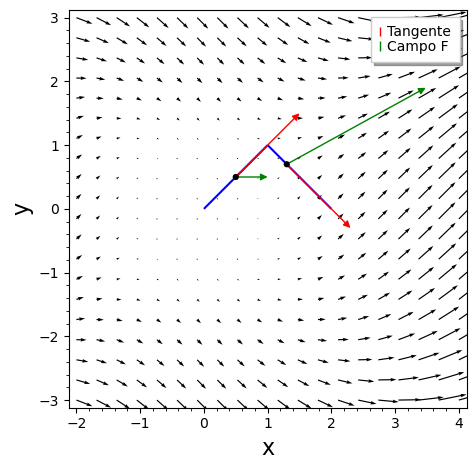
\includegraphics[width=0.25\textwidth]{imagens/lista06/picture_lista06_q01_item04.png}
				\captionof{figure}{Campo vetorial $f$ e caminho $C$}
			\end{center}
		\end{enumerate}
	\end{solucao}
	
	\begin{exercicio}{2}
		(T. Apostol; seção 10.9; exercícios 2 e 8)
		
		\begin{enumerate}
			\item[2.] Encontre a quantidade de trabalho feito pela força $f(x,y)=(x^2-y^2)\textbf{i}+2xy\textbf{j}$ ao mover a partícula (no sentido anti-horário) uma vez ao redor do quadrado limitado pelos eixos de coordenadas e pelas linhas $x=a$ e $y=a$, $a>0$.
			\item[8.] Calcule a integral com respeito ao comprimento de arco $\int_C y^2 ds$, onde $C$ tem a equação vetorial
			\[
			\alpha(t)=a(t-\sin(t))\textbf{i} + a(1-\cos(t))\textbf{j}, 0\leq t\leq 2\pi
			\]
		\end{enumerate}
	\end{exercicio}
	
	\begin{exercicio}{3}
		(T. Apostol; seção 10.13; exercício 6)
		\begin{enumerate}
			\item[6.] Um campo de força $f$ é definido no $\mathbb{R}^3$ pela equação
			\[
			f(x,y,z)=y\textbf{i} + z\textbf{j} +yz\textbf{k}
			\]
			\begin{enumerate}[label=\alph*)]
				\item Determine se $f$ é conservativa ou não.
				\item Calcule o trabalho feito ao mover a partícula pela curva descrita por
				\[
				\alpha(t)=\cos(t)\textbf{i}+\sin(t)\textbf{j}+e^t\textbf{k}
				\]
				Quando $t$ varia de $0$ até $\pi$.
			\end{enumerate}
		\end{enumerate}
	\end{exercicio}
	
	\begin{exercicio}{4}
		(T. Apostol; seção 10.18; exercícios 3 e 9)
		
		Determine se $f$ é gradiente de um campo escalar ou não. Quando $f$ é gradiente, encontre uma função potencial correspondente $\varphi$.
		\begin{enumerate} 
			\item[3.] $f(x,y)=(2xe^y+y)\textbf{i}+(x^2e^y+x=2y)\textbf{j}$.
			\item[9.] $f(x,y,z)=3y^4z^2\textbf{i}+4x^3z^2\textbf{j}-3x^2y^2\textbf{k}$
		\end{enumerate}
	\end{exercicio}
\end{document}